\documentclass{article}
\usepackage{enumerate}
\usepackage{graphicx}
\usepackage{float}

\usepackage{amsmath}
\usepackage[margin=1in]{geometry}
\usepackage[parfill]{parskip}

\newcommand{\heading}[1]{\bigskip \textbf{#1}}
\DeclareMathOperator{\sech}{sech}

\title{Physics 112 Problem Set 2 \\ \large{Holzapfel, Section 102}}
\author{Sahil Chinoy}
\date{September 15, 2017}

\begin{document}
\maketitle{}

\begin{enumerate}

	\item 

	\begin{enumerate}[(a)]

		\item 

		As given in (1.35), $\sigma(s) \simeq \log g(N,0) - 2s^2/N$. But for a spin system in an external magnetic field $B$, the spin excess $s$ is related to the potential energy $U$ by $U(s) = -2smB$, where $m$ is the magnetic moment of each spin (1.5). So

		$$\sigma(U) \simeq \log g(N,0) - U^2/2m^2B^2N.$$

		Then, from the definition of the fundamental temperature (1.26),

		$$\frac{1}{\tau} = \frac{d \sigma}{d U} = \frac{-U}{m^2B^2N}.$$

		Substituting the relationship between spin excess and energy,

		$$\frac{1}{\tau} = \frac{2s}{mBN},$$ which implies the fractional magnetization is

		$$\frac{2s}{N} = \frac{mB}{\tau}.$$

		The relationship between spin excess and energy holds in expectation (it might fluctuate randomly at any given moment), so $U$ denotes $\langle U \rangle$ and $s$ denotes $\langle s \rangle$.

		\item

		\begin{figure}[H]
		\caption{Entropy versus energy}
		\centering
		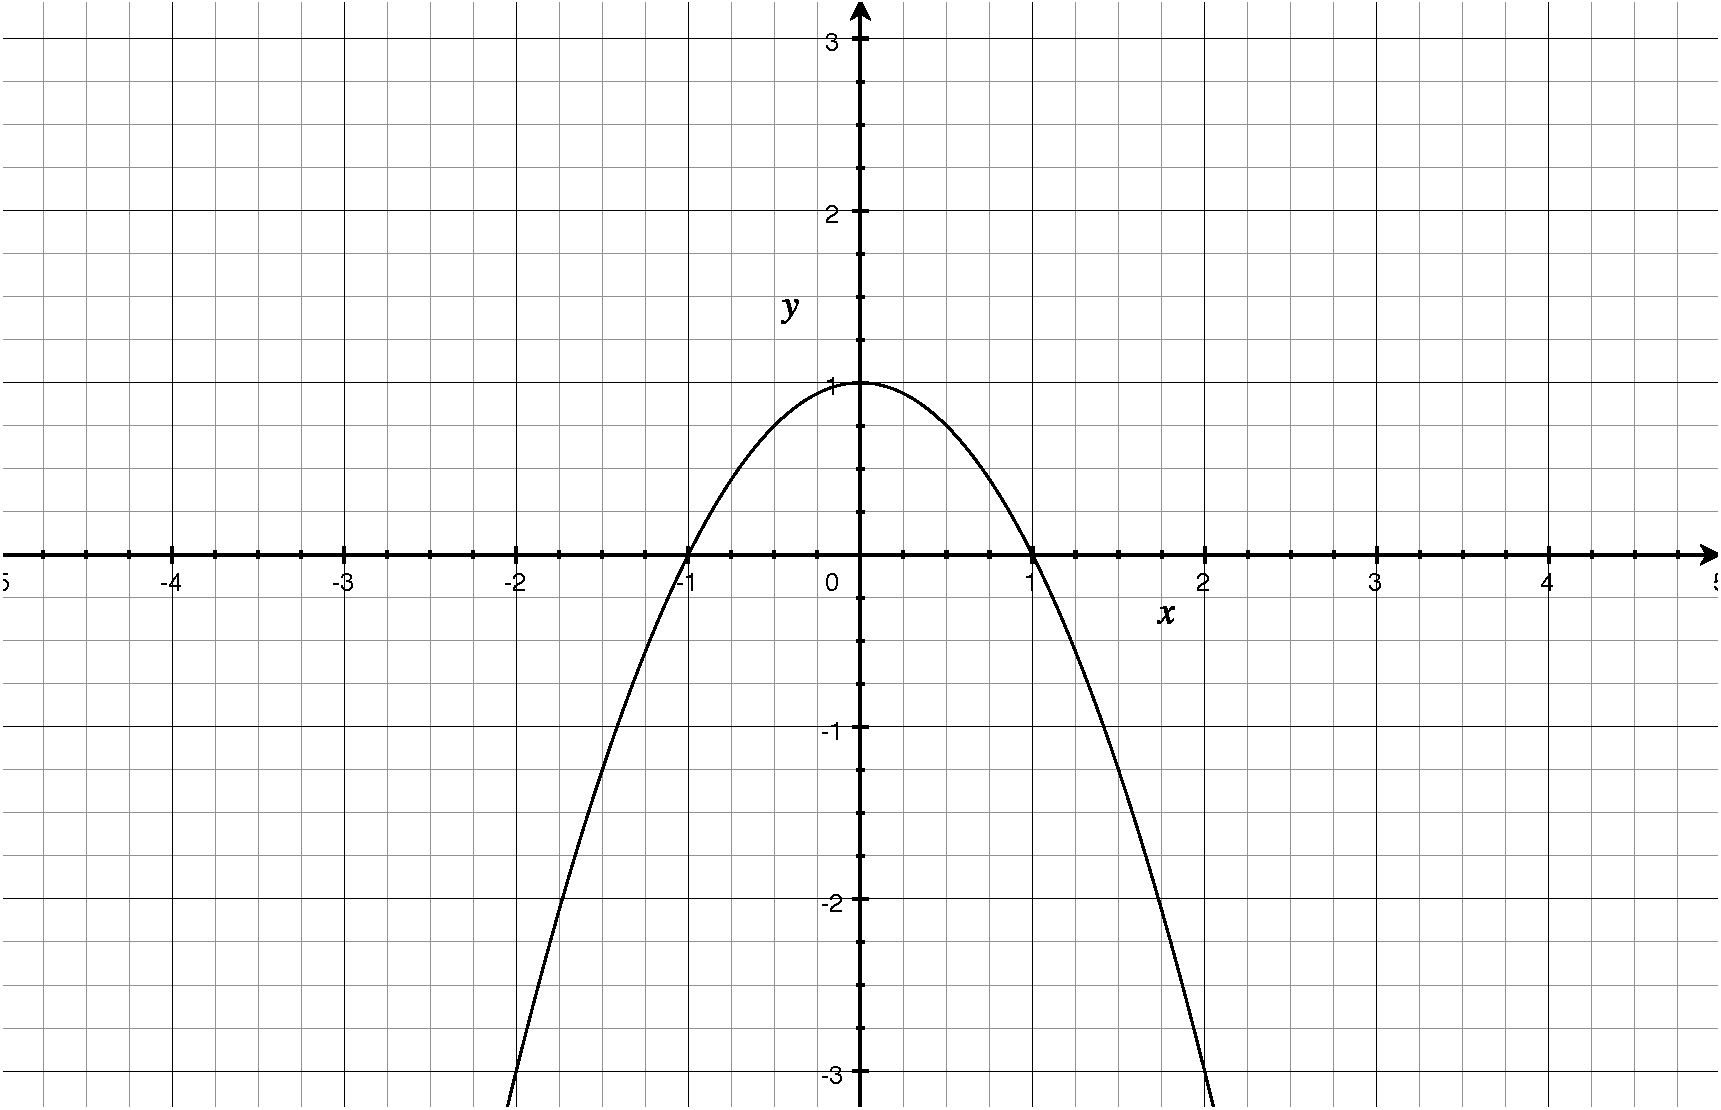
\includegraphics[width=10cm]{img/1-entropy}
		\end{figure}

		\begin{figure}[H]
		\caption{Temperature versus energy}
		\centering
		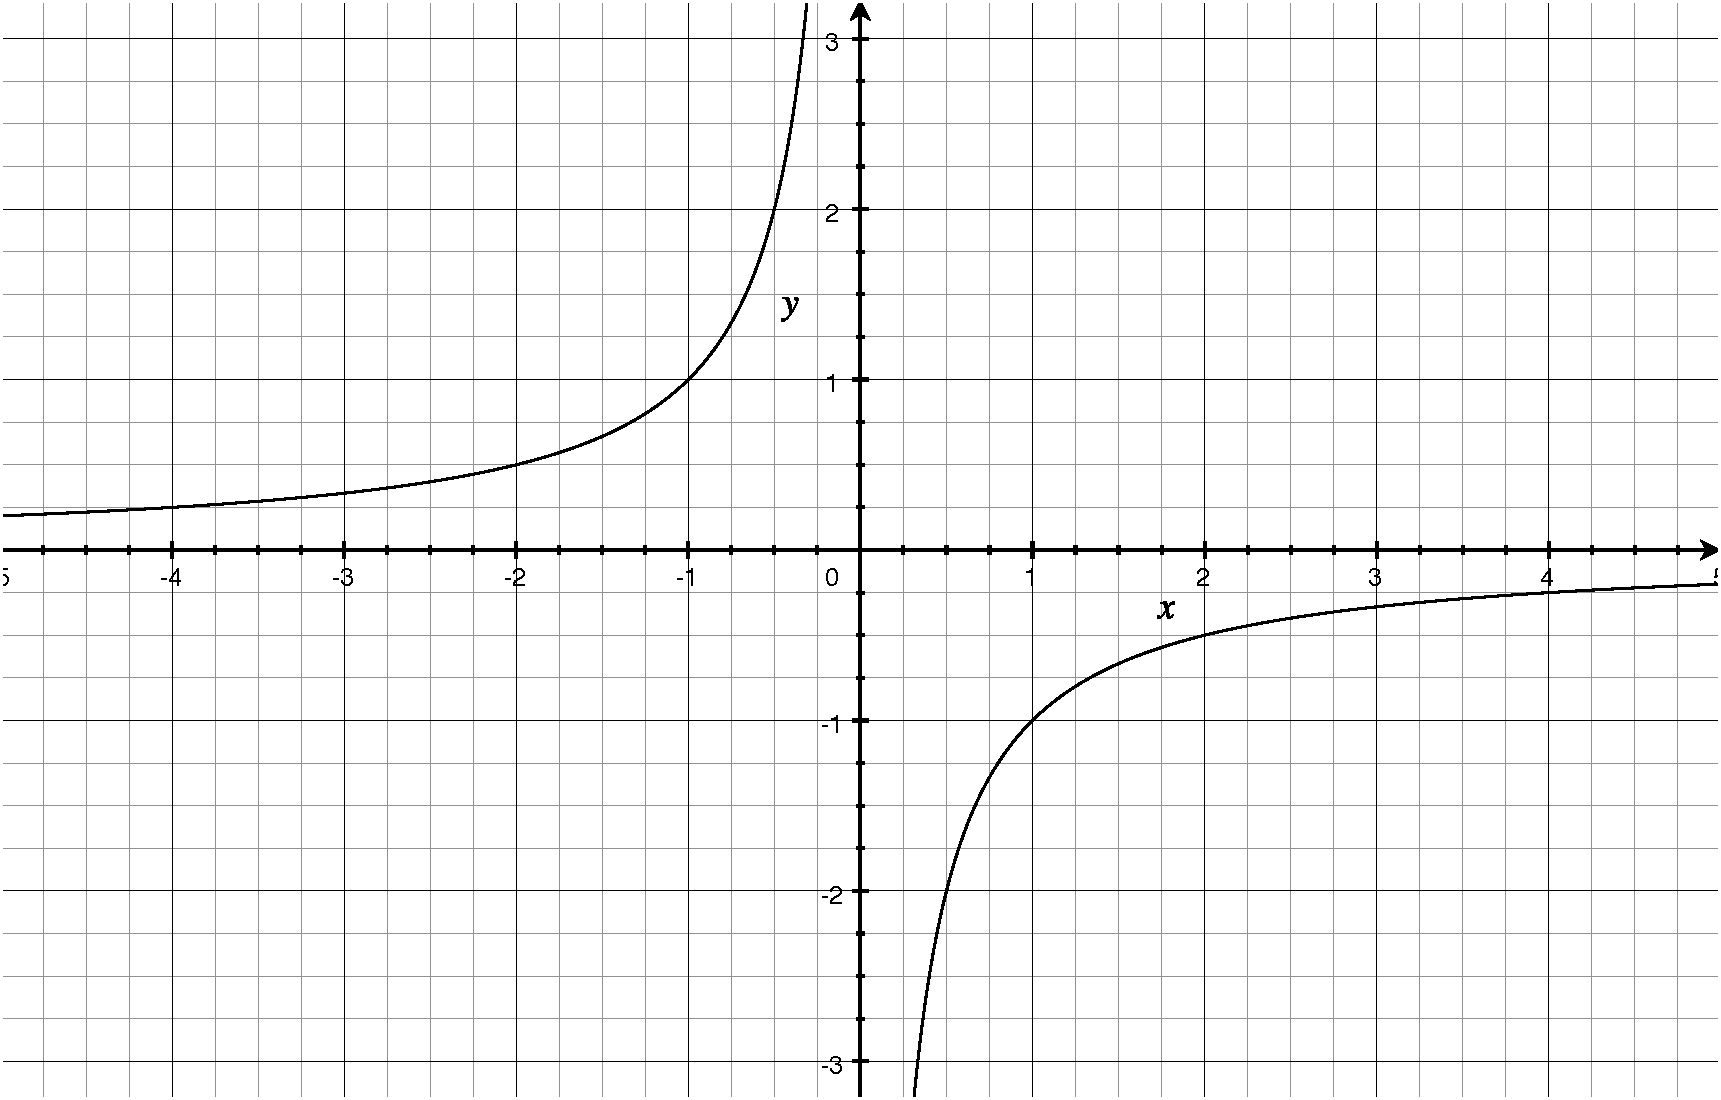
\includegraphics[width=10cm]{img/1-temperature}
		\end{figure}

		Energy would flow from the system with negative temperature to the system with positive temperature. We can see this by noting that a negative temperature implies positive energy, and to move in the direction of increasing entropy, energy must decrease. Likewise, a positive temperature implies negative energy, so to increase entropy, energy must increase.

	\end{enumerate}

	\item

	\begin{enumerate}[(a)]

		\item

		We can think of this as two independent events. First, we choose $M$ atoms to move from the $N$ total atoms. There are ${N \choose M}$ ways to do this. Then, we place each of those $M$ atoms at one of $N$ interstices, and there are again ${N \choose M}$ ways to do this. There are $N$ interstices because we can think of the center of each 8-atom cube as one interstitial site, but each atom is a vertex of 8 distinct cubes, so there are $N$ cubes and $N$ interstitial sites.

		So the total number of ways to take $M$ atoms and place them on $N$ interstices is

		$$g(N, M) = \left[{N \choose M}\right]^2 = \left( \frac{N!}{M!(N-M)!} \right)^2.$$

		\item

		Beginning from the definition of entropy,

		$$\sigma = \log[g(N,M)] = 2[ \log(N!) - \log(M!) - \log((N-M)!) ].$$

		We assume $N \gg 1$ and employ the approximation $\log (N!) \approx N\log N - N$. So

		\begin{align*}
		\sigma &= \log[g(N,M)] = 2[ N\log N - N - M \log M + M - (N-M) \log (N-M) + N - M] \\
		&= 2[ N\log N - M \log M - N \log (N-M) + M \log (N-M)]
		\end{align*}

		Substituting $M = U/\epsilon$, 

		$$\sigma = 2\left[ N\log N - \frac{U}{\epsilon} \log \frac{U}{\epsilon} - N \log (N- \frac{U}{\epsilon}) + \frac{U}{\epsilon} \log (N- \frac{U}{\epsilon}) \right].$$

		Differentiating to get the temperature

		\begin{align*}
		\frac{1}{k_B T} &= \frac{d\sigma}{dU} = 2 \left[ \frac{-1}{\epsilon} \log M - \frac{1}{\epsilon} + \frac{N}{N - M} \frac{1}{\epsilon} + \frac{1}{\epsilon} \log(N - M) - \frac{U}{\epsilon}\frac{1}{N - M}\frac{1}{\epsilon} \right] \\
		\frac{\epsilon}{2 k_B T} &= \log \left( \frac{N-M}{M} \right) = \log \left( \frac{N}{M} - 1 \right).
		\end{align*}

		Rearranging,

		$$\frac{M}{N} = \frac{1}{1 + \exp(\epsilon / 2 k_B T)}.$$

	\end{enumerate}

	\item

	\begin{enumerate}[(a)]

		\item

		The number of ways of taking $M$ atoms from $N$ lattice sites and moving each to one of the $\beta$ sites immediately surrounding its original position is

		$$g(N,M) = \frac{N!}{M! (N-M)!} \beta^M,$$

		so the entropy is 

		$$\sigma = N\log N - M \log M - N \log (N-M) + M \log (N-M) + M \log \beta.$$

		Proceeding as in (2),

		\begin{gather*}
		\sigma =  N\log N - \frac{U}{\epsilon} \log \frac{U}{\epsilon} - N \log (N- \frac{U}{\epsilon}) + \frac{U}{\epsilon} \log (N- \frac{U}{\epsilon}) + \frac{U}{\epsilon} \log \beta \\
		\frac{1}{k_B T} = \frac{d\sigma}{dU} = \frac{1}{\epsilon} \left( -\log M + \log (N-M) + \log \beta \right) \\
		\frac{\epsilon}{k_B T} = \log \left[ \beta \left( \frac{N-M}{M} \right) \right], 
		\end{gather*}

		Rearranging,

		\begin{gather*}
		\beta \left( \frac{N}{M} - 1 \right) = \exp \left( \frac{\epsilon}{k_B T} \right) \\
		\beta \frac{N}{M} = \exp ( \epsilon / k_B T) + \beta \\
		\frac{M}{N} = \frac{\beta}{\exp ( \epsilon / k_B T) + \beta }.
		\end{gather*}

		\item

		\begin{enumerate}[i)]

			\item

			As $\beta \to \infty$, $M/N \to 1$. As $\beta$ increases, it becomes increasingly ``easy'' to displace an atom in the sense that there are more ways to do so, and given the assumption that all microstates are equally probable, this means that the probability that we will find an atom in a displaced state approaches 1.

			\item

			As $T \to \infty$, $M/N \to \beta/(1 + \beta) \simeq 1$ for sufficiently large $\beta$. As the thermal energy in the system increases, there is sufficient energy to excite a majority of the $N$ atoms.

			\item

			As $T \to 0$, $M/N \to 0$. At absolute zero, there is no energy available to displace any of the $N$ atoms.

		\end{enumerate}

	\end{enumerate}

	\item

	\begin{enumerate}[(a)]

		\item

		Starting with the multiplicity function of a system of $N$ spins with spin excess $s$,

		$$g(N,s) = \frac{N!}{(N/2 + s)! (N/2 - s)!}.$$

		Then

		$$\sigma(N, s) = \log g(N,s) = \log (N!) - \log [(N/2 + s)!] -  \log [(N/2 - s)!].$$

		Under the assumption $N \gg 1$, we approximate $N! \simeq N \log N - N$. Define $a = 2s/N$, and recall that $U = -2smB$, so $a = -U/NmB$. So

		\begin{align*}
		\sigma(N, a) &= N \log N - N \\
		&- N \left( \frac{1+a}{2} \right) \log \left[ N \left( \frac{1+a}{2} \right) \right] + N \left( \frac{1+a}{2} \right) \\ 
		&- N \left( \frac{1-a}{2} \right) \log \left[ N \left( \frac{1-a}{2} \right) \right] + N \left( \frac{1-a}{2} \right) \\
		&= -N \left[ \left( \frac{1+a}{2} \right) \log \left( \frac{1+a}{2} \right) + \left( \frac{1-a}{2} \right) \log \left( \frac{1-a}{2} \right)\right].
		\end{align*}

		Differentiating,

		\begin{align*}
		\frac{\partial \sigma}{\partial U} &=  \frac{\partial \sigma}{\partial a} \frac{\partial a}{\partial U} = \frac{\partial \sigma}{\partial a} \left( \frac{-1}{NmB} \right) \\
		&= -N \left[ \frac{1}{2} \log \left( \frac{1+a}{2} \right) - \frac{1}{2} \log \left( \frac{1-a}{2} \right) \right] \left( \frac{-1}{NmB} \right) \\
		&= \frac{1}{2mB} \log \left( \frac{1+a}{1-a} \right).
		\end{align*}

		Now, since $\partial \sigma / \partial U = 1 / k_B T$, we can write $a$ in terms of temperature, defining $x = mB /k_B T$,

		\begin{gather*}
		\log \left( \frac{1+a}{1-a} \right) = \frac{2mB}{k_B T} = 2x \\
		\frac{1+a}{1-a} = e^{2x} \\
		a = \frac{e^{2x} - 1}{e^{2x} + 1} = \tanh x.
		\end{gather*}

		Substituting this expression back into the expression for entropy,

		\begin{align*}
		\sigma(N, x) &= -N \left[ \left( \frac{1 + \tanh x}{2} \right) \log \left( \frac{1 + \tanh x}{2} \right) + \left( \frac{1 - \tanh x}{2} \right) \log \left( \frac{1 - \tanh x}{2} \right)  \right] \\
		&= -\frac{N}{2} \left[ \log (1-\tanh ^2 x) - \log 4 + \left( \tanh x \right) \log \left( \frac{1+\tanh x}{1-\tanh x} \right) \right] \\
		&= -\frac{N}{2} \left[ \log (\sech ^2 x) - \log 4 + \left( \tanh x \right) \log e^{2x} \right] \\
		&= N [ \log(2 \cosh x) - x \tanh x ].
		\end{align*}

		Thus, since $S$ and $\sigma$ differ only by a factor of $k_B$,

		$$ S = N k_B [ \log(2 \cosh x) - x \tanh x ].$$

		\item

		\begin{figure}[H]
		\caption{$S/Nk_B$ versus $k_B T / mB$}
		\centering
		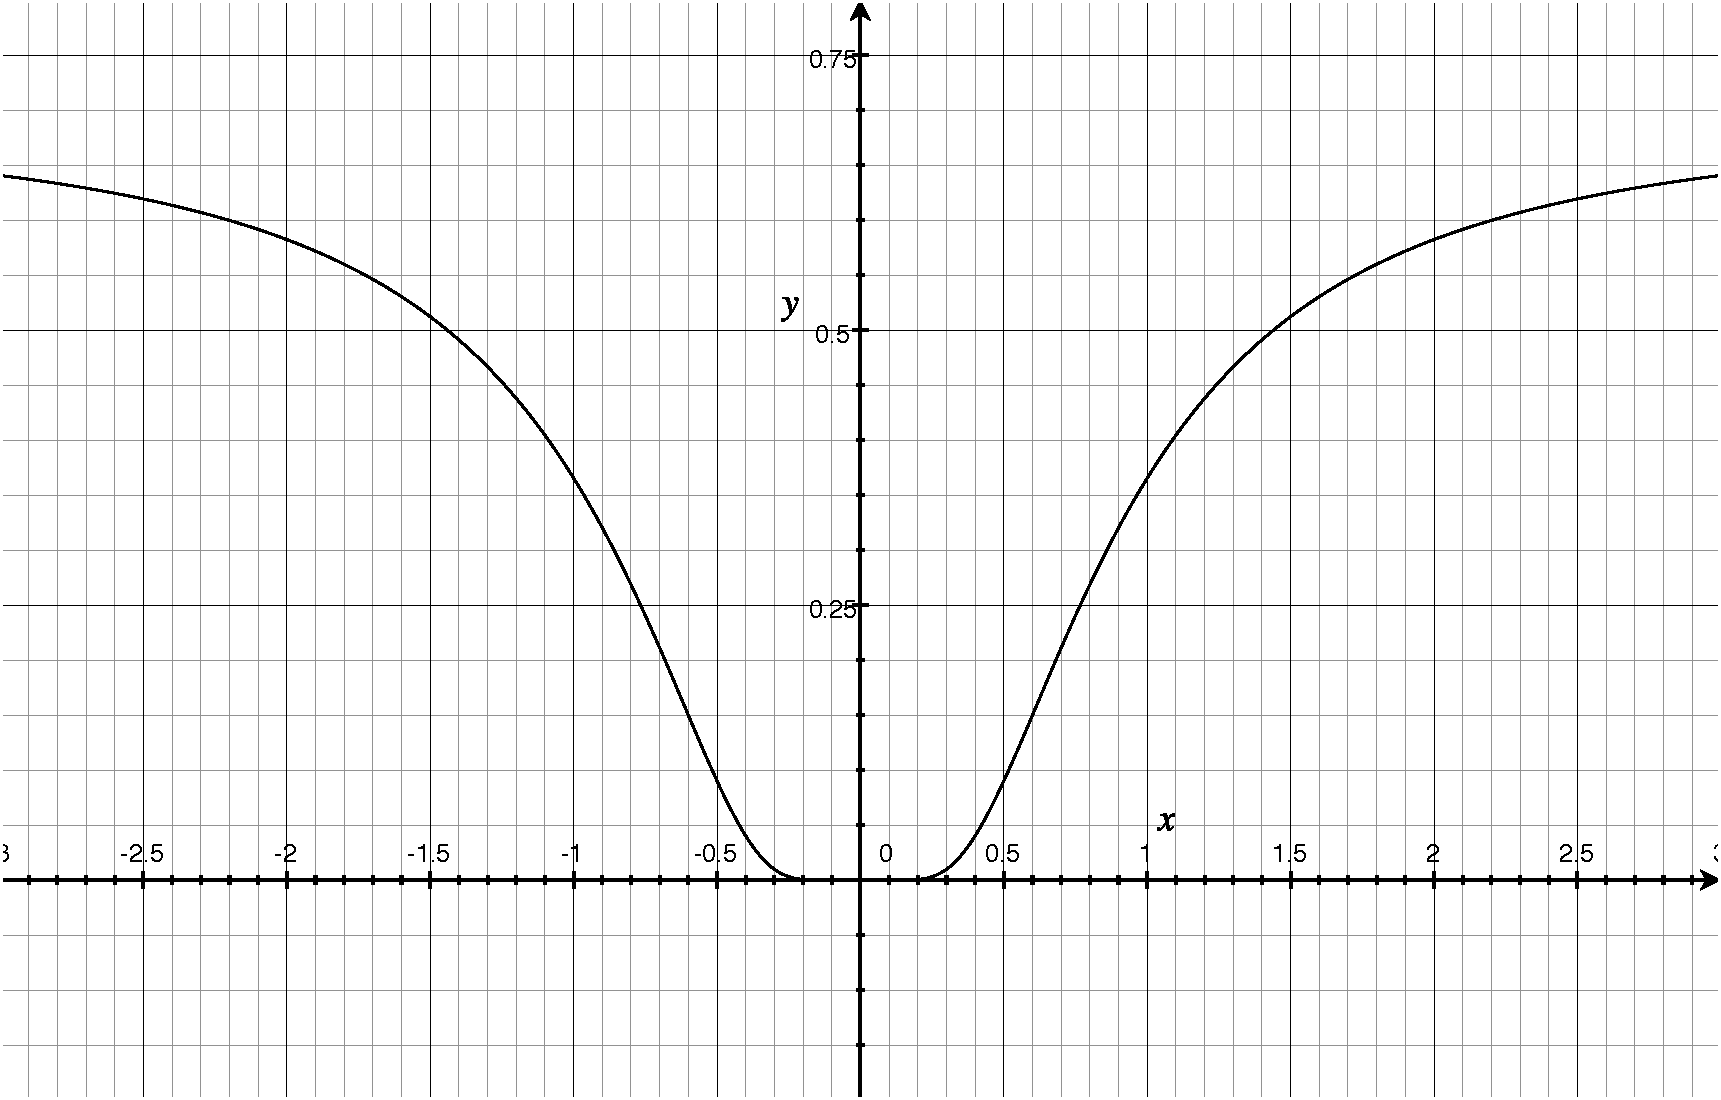
\includegraphics[width=10cm]{img/4-entropy}
		\end{figure}

		We see that $S \to 0$ (a minimum) as $T \to 0$, as required by the third law of thermodynamics -- this corresponds to freezing the dipoles into alignment. Further, as $T \to \pm \infty$, $S \to N k_B \log 2$, which is the maximum entropy state that occurs when exactly half of the spins are up and half are down. We can approach this state from the left (all spins originally aligned with the magnetic field) or from the right (all spins originally aligned against the magnetic field).

		In this case, negative temperatures refer to the states where more than half of the spins are aligned against the magnetic field, so increasing energy decreases entropy (the opposite of what we usually see).

	\end{enumerate}

	\item

	\begin{enumerate}[(a)]

		\item

		For $N \gg 1$ and $q \gg 1$, $(q + N - 1) \approx (q + N)$ and $(N-1) \approx N$. Now, we use the Stirling approximation $N! \approx (2 \pi N)^{1/2} N^N \exp(-N)$ to find

		\begin{gather*}
		g(N,q) \approx \frac{(q+N)!}{q! N!} = \frac{(2 \pi (q+N))^{1/2} (q+N)^{q+N} \exp(-q-N)}{(2 \pi q)^{1/2} q^q \exp(-q) \; (2 \pi N)^{1/2} N^N \exp(-N)} \\
		g(N,q) \approx \sqrt{\frac{q+N}{2\pi qN}} \left( \frac{q+N}{q} \right)^q \left( \frac{q+N}{N} \right)^N.
		\end{gather*}

		And for large $q$ and $N$, $\sqrt{(q+N)/qN} \approx 1$, so

		$$g(N,q) \approx \left( \frac{q+N}{q} \right)^q \left( \frac{q+N}{N} \right)^N.$$

		\item

		Taking the log to find the entropy,

		$$
		\sigma(N, q) = \log g(N,q) = (q+N)\log (q+N) - q \log q - N \log N.
		$$

		Note that if we had not ignored the factor of $\sqrt{(q+N) / 2\pi qN}$ in the original expression, we would have had

		$$
		\sigma(N, q) = \log g(N,q) = (q+N + 1/2)\log (q+N) - (q + 1/2) \log q - (N + 1/2) \log N - (1/2) \log 2 \pi,
		$$

		which in the limit of large $q$ and $N$ is very close to the original expression.

		\item

		Differentiating to find the temperature,

		\begin{gather*}
		\frac{1}{k_BT} = \frac{\partial \sigma}{\partial U} = \frac{\partial \sigma}{\partial q} \frac{\partial q}{\partial U} = \frac{1}{\epsilon} \left( \log (q+N) + 1 - \log q - 1 \right) \\
		\frac{1}{T} = \frac{k_B}{\epsilon} \log \left( \frac{q+N}{q} \right) \\
		T = \frac{\epsilon}{k_B \log ((q+N) / q)},
		\end{gather*}

		or in terms of energy,

		$$T(U) = \frac{\epsilon}{k_B \log ((U + N\epsilon) / U )}.$$

		\item

		Rearranging,

		\begin{gather*}
		\log \left( \frac{U + N\epsilon} {U} \right) = \frac{\epsilon}{k_B T} \\
		1 + \frac{N\epsilon}{U} = \exp(\epsilon/k_BT) \\
		U = \frac{N\epsilon}{\exp(\epsilon/k_BT) - 1}.
		\end{gather*}

		\item

		Let $x = \epsilon / k_B T$. Then 

		\begin{gather*}
		C = \frac{\partial U}{\partial T} = \frac{\partial U}{\partial x} \frac{\partial x}{\partial T} = \frac{-N \epsilon \; e^x}{(e^x - 1)^2} \frac{-\epsilon}{k_B T^2} = \frac{N \epsilon^2}{k_B T^2} \frac{e^x}{(e^x -1)^2} = Nk_B \frac{x^2 \; e^x}{(e^x -1)^2}.
		\end{gather*}

		As $T \to \infty, x \to 0$. We use L'Hospital's rule twice to find the heat capacity in this limit: 

		$$\lim_{x \to 0} C(x) = \lim_{x \to 0} N k_B \frac{2x e^x + x^2 e^x}{2(e^x - 1)} = \lim_{x \to 0} N k_B \frac{2 e^x + 4x e^x + x^2 e^x}{2e^x} = N k_B.$$

		\item

		\begin{figure}[H]
		\caption{$C/Nk_B$ versus $k_B T / \epsilon$ for $\epsilon = 1, 2$}
		\centering
		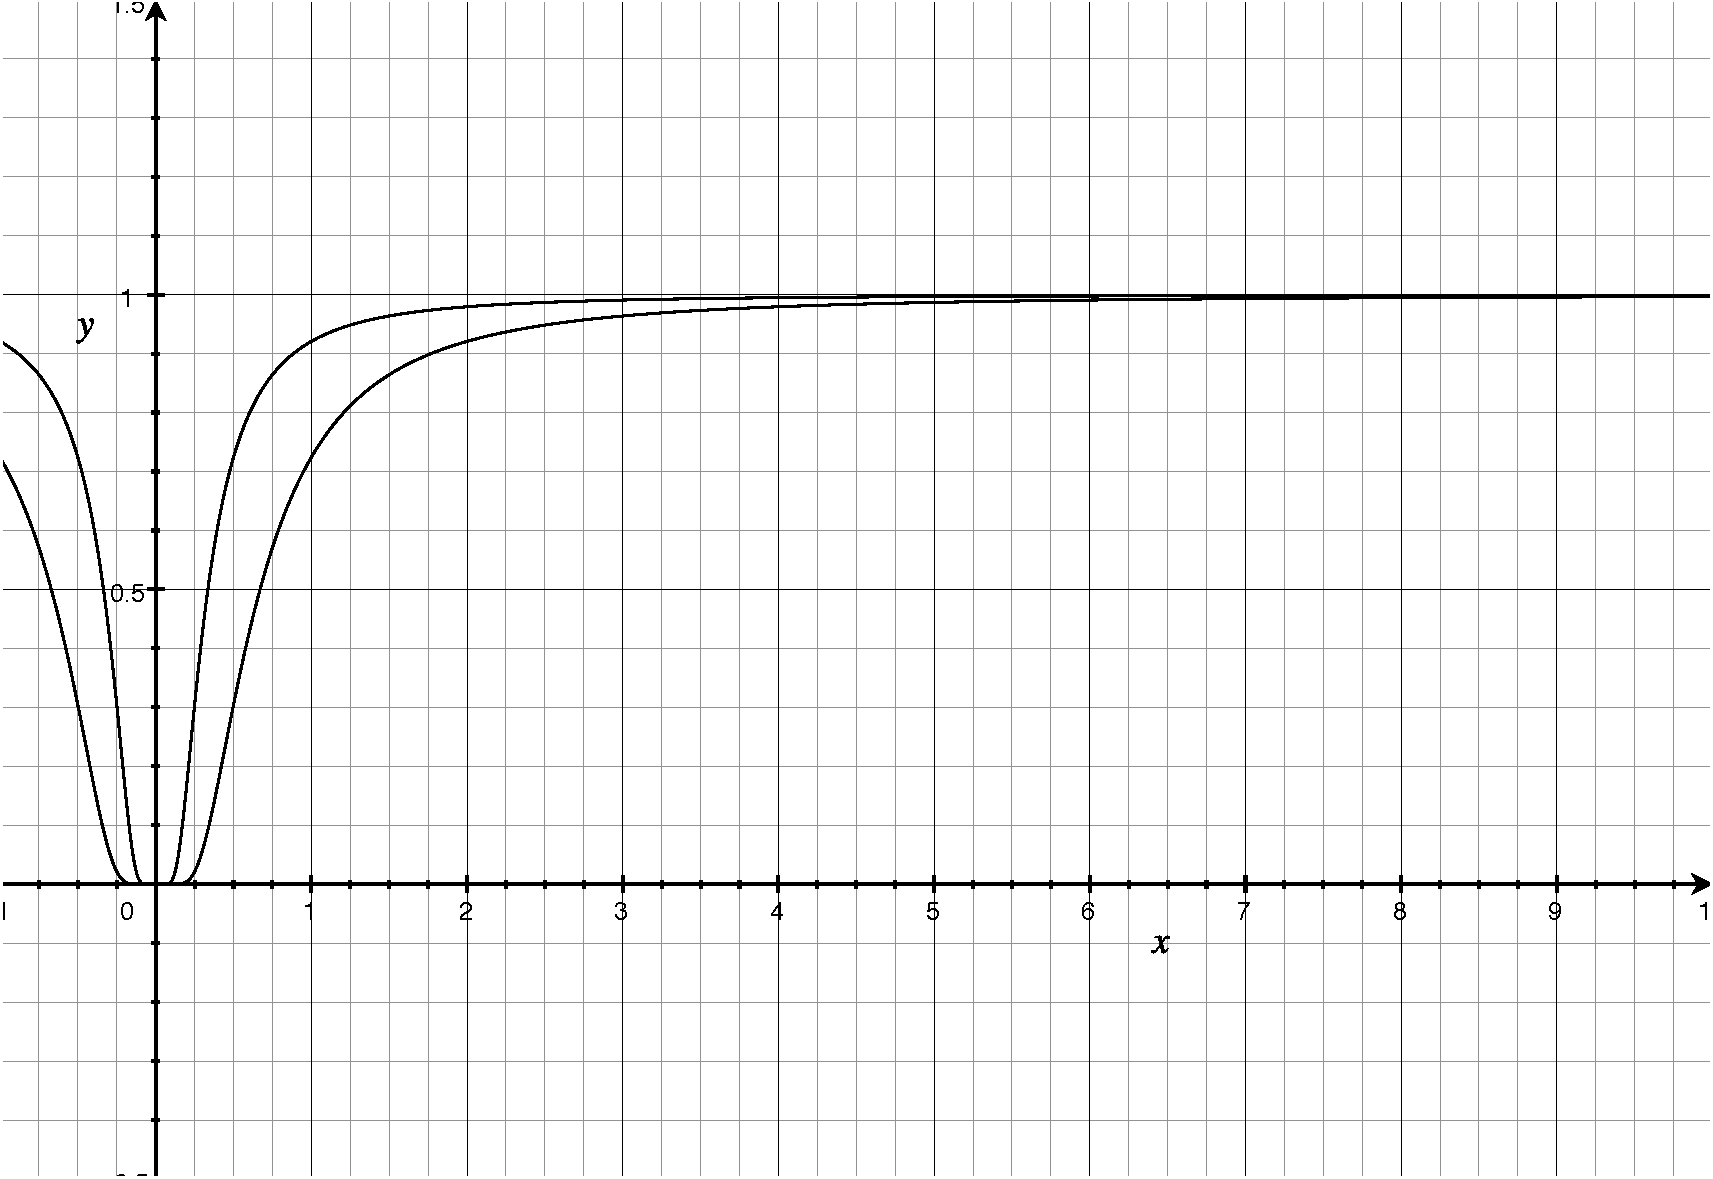
\includegraphics[width=10cm]{img/5-heatcapacity}
		\end{figure}

		The heat capacity for diamond, a hard material, is smaller than the heat capacity for lead (for low temperatures). We can see this because the curve for higher $\epsilon$ lies below the curve for lower $\epsilon$, and we can think of diamond (whose atoms are tightly bound together; i.e. each oscillator vibrates quickly, with more energy) as a material with a higher value for $\epsilon$ than lead.

		At low temperatures, the quantum energy levels for diamond are sufficiently spread out so that many energy levels are too large in value to be populated, which means more atoms are excited and thus temperature rises faster for the same amount of applied heat.

		\item

		Looking up the Laurent series expansion,

		$$\frac{e^x}{(e^x -1)^2} = \frac{1}{x^2} - \frac{1}{12} + \mathcal{O}(x^2).$$

		So

		$$C = Nk_B \left(1 - \frac{x^2}{12} + \mathcal{O}(x^4) \right).$$

		For large $T$, we consider terms to second order in $\epsilon/k_B T$, so

		$$C \approx Nk_B \left[1 - \frac{1}{12} \left(\frac{\epsilon}{k_B T}\right)^2 \right].$$


	\end{enumerate}

	\item

	\begin{enumerate}[(a)]

		\item

		For the reservoir, $\Delta S_{res} = \Delta Q / T = - C \Delta T / T = -(4.2 \text{ kJ/K}) \times (100 \text{ K}) / 373 \text{ K} = -1.1 \text{ kJ/K}$, since it does not change temperature.

		For the water, 
		$$\Delta S_{water} = \int \frac{dQ}{T} = C \int\limits_{T_i}^{T_f} \frac{dT} {T} = C [ \log (T_f) - \log (T_i) ],$$

		for $C = 4.2 \text{ kJ/K}$, $T_i = 273 \text{ K}$, $T_f = 373 \text{ K}$, so $\Delta S_{water} = (4.2 \text{ kJ/K})  \log (373 \text{ K}/ 273 \text{ K}) = 1.3 \text{ kJ/K}$.

		So the entropy change of the universe is $\Delta S = \Delta S_{water} + \Delta S_{res} = 1.3 \text{ kJ/K} - 1.1 \text{ kJ/K} = 0.2 \text{ kJ/K}$.

		\item

		$S = k_B \log g$, so $\Delta S = k_B [\log g_f - \log g_i] = k_B \log (g_f / g_i)$. From (a), $\Delta S = C \log (T_f / T_i)$. So $g_f / g_i = (T_f / T_i)^{C/k_B}$, or

		$$
		\frac{g_f} {g_i} = \left( \frac{373 \text{ K}}{273 \text{ K}} \right) ^ {\frac{4.2 \text{ kJ/K}}{1.3 \times 10^{-26} \text{ kJ/K}}} \approx 10^{10^{26}}.
		$$

		\item

		The entropy change of the two reservoirs is 
		$$
		\Delta S_{res} = \Delta S_1 + \Delta S_2 = -[(4.2 \text{ kJ/K}) \times (50 \text{ K})] \left( \frac{1} {373 \text{ K}} + \frac{1} {323 \text{ K}} \right) = -1.2 \text{ kJ/K}.
		$$

		The entropy change of the water is the same: 
		$$
		\Delta S_{water} = \Delta S_1 + \Delta S_2 = (4.2 \text{ kJ/K}) \left[ \log \left( \frac{323 \text{ K}}{273 \text{ K}} \right) + \log \left( \frac{373 \text{ K}}{323 \text{ K}} \right) \right] = 1.3 \text{ kJ/K}.
		$$

		So the entropy change of the universe is $\Delta S = \Delta S_{water} + \Delta S_{res} = 1.3 \text{ kJ/K} - 1.2 \text{ kJ/K} = 0.1 \text{ kJ/K}$.

		\item

		We can see that if we continue the subdivision into infinite steps, we would approach $\Delta S = 0$ for the universe. This implies that the process is reversible in this limit, since if the entropy change of the process were truly zero, then reversing it does not violate the second law of thermodynamics.

	\end{enumerate}

\end{enumerate}

\end{document}